% Copyright (c) 2015 Daniele Masini - d.masini.it@gmail.com

\section{Esercizi}

\subsection{Esercizi dei singoli paragrafi}

\begingroup
\hypersetup{linkcolor=black}
\subsubsection*{\ref{sect:primo_teorema_angolo_esterno} - \nameref{sect:primo_teorema_angolo_esterno}}
\endgroup

\begin{esercizio}
\label{ese:3.1}
Vero o falso? In un triangolo:
\begin{enumeratea}
\item Per ogni lato c'è un solo angolo esterno\hfill\boxV\quad\boxF
\item Un angolo esterno è maggiore della somma degli angoli interni\hfill\boxV\quad\boxF
\item L'angolo esterno non può essere acuto\hfill\boxV\quad\boxF
\item L'angolo esterno è maggiore di ciascuno dei tre angoli interni\hfill\boxV\quad\boxF
\item L'angolo interno è minore di ciascuno degli angoli esterni non adiacenti\hfill\boxV\quad\boxF
\item L'angolo esterno è maggiore di ciascuno degli angoli interni ad esso non adiacenti\tab\tab\hfill\boxV\quad\boxF
\end{enumeratea}
\end{esercizio}

\begin{esercizio}
\label{ese:3.2}
Per ciascun vertice del triangolo nella figura~\ref{fig:ese3.2} disegna un angolo esterno.
\end{esercizio}

\begin{figure}[htb]
\centering% Copyright (c) 2015 Daniele Masini - d.masini.it@gmail.com

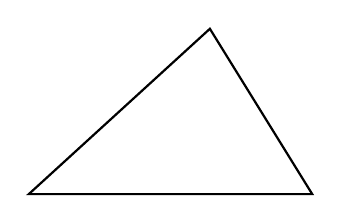
\begin{tikzpicture}[scale=1,font=\small]
\usetikzlibrary{calc, through, intersections}

\begin{scope}
\coordinate (a) at (0,0);
\coordinate (b) at (-2.3,-2.1);
\coordinate (c) at (1.3,-2.1);
%\draw[fill=gray!10] (a) -- (b) -- (c) -- cycle;

%\draw[thick] (a) node[above] {$A$} -- (b) node[left] {$B$} -- (c) node[right] {$C$} -- cycle;
\draw[thick] (a) -- (b) -- (c) -- cycle;

\end{scope}

\end{tikzpicture}

\caption{Esercizio~\ref{ese:3.2}}\label{fig:ese3.2}
\end{figure}

\begin{esercizio}
\label{ese:3.3}
Nel triangolo isoscele $ABC$ di base $AB$ prolunga il lato $CB$ fino a un punto $D$. Dimostra che: $A\widehat{B}D>A\widehat{C}B$, $C\widehat{B}A>A\widehat{D}B$, $C\widehat{A}B>B\widehat{A}D$, $C\widehat{A}B>B\widehat{D}A$.
\end{esercizio}

\begin{esercizio}
\label{ese:3.4}
Internamente a un triangolo $ABC$ prendi un punto $D$. Congiungi $D$ con $A$, con $B$ e con $C$. Il prolungamento di $AE$ incontra il lato $BC$ nel punto $E$. Dimostra che: $B\widehat{D}E>B\widehat{A}D$, $B\widehat{D}C>B\widehat{A}C$, $A\widehat{E}B>C\widehat{D}B$.
\end{esercizio}

\begin{esercizio}
\label{ese:3.5}
Nel triangolo $ABC$ traccia la bisettrice $AP$ dell'angolo in $A$. Dimostra che nel triangolo $APC$, l'angolo in $P$ è maggiore dell'angolo in $A$.
\end{esercizio}

\begin{esercizio}
\label{ese:3.6}
Dimostra che la somma di due angoli interni di un triangolo è minore di un angolo piatto. (Considera l'angolo esterno a uno dei due angoli).
\end{esercizio}

\begin{esercizio}
\label{ese:3.7}
Dimostra che un triangolo non può avere più di due angoli retti.
\end{esercizio}

\begin{esercizio}
\label{ese:3.8}
Dimostra che un triangolo non può avere due angoli ottusi.
\end{esercizio}

\begin{esercizio}
\label{ese:3.9}
Dimostrare che gli angoli alla base di un triangolo isoscele devono essere acuti.
\end{esercizio}

\begingroup
\hypersetup{linkcolor=black}
\subsubsection*{\ref{sect:rette_perpendicolari} - \nameref{sect:rette_perpendicolari}}
\endgroup

\begin{esercizio}
\label{ese:3.10}
Vero o falso?
\begin{enumeratea}
\item Dati un punto $P$ e una retta $r$ esiste sempre una retta perpendicolare a $r$ e passante per $P$\tab\hfill\boxV\quad\boxF
\item Dati un punto $P$ e una retta $r$ esistono infinite rette passanti per $P$ e perpendicolari a $r$\tab\hfill\boxV\quad\boxF
\item L'unicità della perpendicolare per un punto a una retta è un assioma\hfill\boxV\quad\boxF
\item L'unicità della parallela per un punto a una retta è un assioma\hfill\boxV\quad\boxF
\end{enumeratea}
\end{esercizio}

\begin{esercizio}
\label{ese:3.11}
Una retta $a$ è perpendicolare a una retta $b$, la quale a sua volta è perpendicolare a una terza retta $c$. Tra loro, le rette $a$ e $c$ sono:
\[\text{a) parallele;\qquad b) perpendicolari;\qquad c) né parallele né perpendicolari.}\]
\end{esercizio}

\begin{esercizio}
\label{ese:3.12}
Disegna le rette passanti per $P$ e perpendicolari alle altre rette presenti nella figura~\ref{fig:ese3.12}.
\end{esercizio}
\begin{figure}[htb]
\centering% Copyright (c) 2015 Daniele Masini - d.masini.it@gmail.com

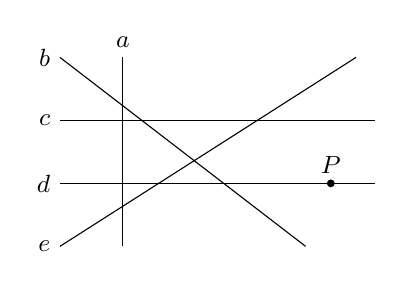
\begin{tikzpicture}[scale=0.8,font=\small]
\usetikzlibrary{calc, through, intersections}

\begin{scope}
\draw (0,0) coordinate (d1) node[left] {$d$} -- (5,0) coordinate (d2);
\draw (0,1) coordinate (c1) node[left] {$c$} -- (5,1) coordinate (c2);
\draw (1,-1) coordinate (a1) -- (1,2) coordinate (a2) node[above] {$a$};
\draw (0,2) coordinate (b1) node[left] {$b$} -- (3.9,-1) coordinate (c2);
\draw (0,-1) coordinate (e1) node[left] {$e$} -- (4.7,2) coordinate (e2);
\draw[fill] (4.3,0) circle (1.5pt) coordinate (p) node[above] {$P$};

%\draw[thick] (a) node[above] {$A$} -- (b) node[left] {$B$} -- (c) node[right] {$C$} -- cycle;

\end{scope}

\end{tikzpicture}

\caption{Esercizio~\ref{ese:3.12}}\label{fig:ese3.12}
\end{figure}

\begin{esercizio}
\label{ese:3.13}
Per ognuno dei punti di intersezione delle tre rette nella figura~\ref{fig:ese3.13} traccia la perpendicolare a ciascuna retta (aiutati con una squadretta).
\end{esercizio}
\begin{figure}[htb]
\centering% Copyright (c) 2015 Daniele Masini - d.masini.it@gmail.com

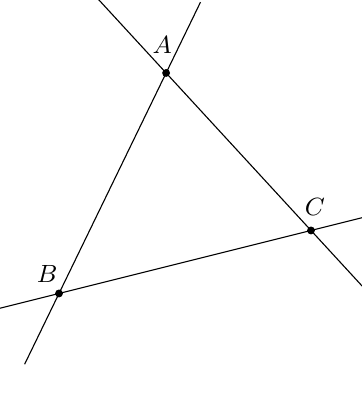
\begin{tikzpicture}[scale=0.8,font=\small, extended line/.style={shorten >=-#1,shorten <=-#1}, extended line/.default=1cm]
\usetikzlibrary{calc, through, intersections}

\begin{scope}
\coordinate (a) at (1.7,3.5);
\coordinate (b) at (0,0);
\coordinate (c) at (4,1);

\draw[extended line=1.5cm] (b) -- (c);
\draw[extended line] (a) -- (b);
\draw[extended line=1.3cm] (a) -- (c);

\draw[fill] (a) circle (1.5pt) node[shift={(-0.05,0.35)}] {$A$};
\draw[fill] (b) circle (1.5pt) node[shift={(-0.15,0.25)}] {$B$};
\draw[fill] (c) circle (1.5pt) node[shift={(0.05,0.3)}] {$C$};

%\path (a) circle (1);
%\path (b) circle (1);
%\path (c) circle (1.5);
\node at (0,-1) {};

%\draw[thick] (a) node[above] {$A$} -- (b) node[left] {$B$} -- (c) node[right] {$C$} -- cycle;

\end{scope}

\end{tikzpicture}

\caption{Esercizio~\ref{ese:3.13}}\label{fig:ese3.13}
\end{figure}

\begin{esercizio}
\label{ese:3.14}
Dimostra che le bisettrici di due angoli adiacenti sono perpendicolari.
\end{esercizio}

\begingroup
\hypersetup{linkcolor=black}
\subsubsection*{\ref{sect:rette_parallele} - \nameref{sect:rette_parallele}}
\endgroup

\begin{esercizio}
\label{ese:3.15}
Vero o Falso?
\begin{enumeratea}
\item Due rette parallele tagliate da una trasversale formano quattro angoli alterni interni\tab\hfill\boxV\quad\boxF
\item Gli angoli corrispondenti sono a due a due interni o esterni\hfill\boxV\quad\boxF
\item Gli angoli interni si trovano da parti opposte rispetto alla trasversale\hfill\boxV\quad\boxF
\item Gli angoli esterni si trovano da parti opposte rispetto alla trasversale\hfill\boxV\quad\boxF
\item Due rette parallele possono anche coincidere\hfill\boxV\quad\boxF
\item La relazione di parallelismo tra rette è una relazione di equivalenza\hfill\boxV\quad\boxF
\item Due rette distinte hanno sempre un punto in comune\hfill\boxV\quad\boxF
\item Una retta che incontra due rette parallele forma angoli alterni interni supplementari\tab\hfill\boxV\quad\boxF
\item Per ogni retta è possibile tracciare una sola retta parallela\hfill\boxV\quad\boxF
\item Se due rette formano con una trasversale due angoli alterni interni allora sono parallele\tab\hfill\boxV\quad\boxF
\item Nel ragionamento per assurdo si nega l'ipotesi per dimostrare che la tesi è vera\tab\tab\hfill\boxV\quad\boxF
\item Ragionando per assurdo si nega la tesi e si ottenere una contraddizione con l'ipotesi\tab\hfill\boxV\quad\boxF
\end{enumeratea}
\end{esercizio}

\begin{esercizio}
\label{ese:3.16}
Nella figura~\ref{fig:ese3.16} disegna una parallela e una perpendicolare alla retta $r$ passanti per $P$ e una parallela e una perpendicolare a $s$ passanti per $Q$.
\end{esercizio}
\begin{figure}[htb]
\centering% Copyright (c) 2015 Daniele Masini - d.masini.it@gmail.com

\begin{tikzpicture}[scale=0.9,font=\small, extended line/.style={shorten >=-#1,shorten <=-#1}, extended line/.default=1cm]
\usetikzlibrary{calc, through, intersections}

\begin{scope}
\clip (-0.2,-0.1) rectangle (8.2,2.8);
\coordinate (p) at (3,0.3);
\coordinate (q) at (4.5,0.5);

\draw (0,0) node[above] {$r$} -- (5,3);
\draw (3,3) -- (8,0) node[above] {$s$};

\draw[fill] (p) circle (1.5pt) node[below] {$P$};
\draw[fill] (q) circle (1.5pt) node[below] {$Q$};

\end{scope}

\end{tikzpicture}

\caption{Esercizio~\ref{ese:3.16}}\label{fig:ese3.16}
\end{figure}

\begin{esercizio}
\label{ese:3.17}
Nella figura~\ref{fig:ese3.17} sono state tracciate due rette parallele e una trasversale. Indica con un arco gli angoli corrispondenti.
\end{esercizio}
\begin{figure}[htb]
\centering% Copyright (c) 2015 Daniele Masini - d.masini.it@gmail.com

\begin{tikzpicture}[scale=0.9,font=\small, extended line/.style={shorten >=-#1,shorten <=-#1}, extended line/.default=1cm]
\usetikzlibrary{calc, through, intersections}

\begin{scope}
\coordinate (p) at (3,0.2);
\coordinate (q) at (4.5,0.5);

\draw (0,0) -- (5,0.5);
\draw (0,1.2) -- (5,1.7);
\draw (1.5,-0.6) -- (3.5,2.4);

\end{scope}

\end{tikzpicture}

\caption{Esercizio~\ref{ese:3.17}}\label{fig:ese3.17}
\end{figure}

\begin{esercizio}
\label{ese:3.18}
Nella figura a fianco sono state tracciate due rette parallele e una trasversale, sapendo che $\alpha=\frac{1}{3}\pi$, dove $\pi$ è l'angolo piatto, indica che frazione dell'angolo piatto sono gli altri angoli:\\
\noindent\begin{minipage}{.5\textwidth}
$\alpha=\frac{1}{3}\pi$\tab\tab $\beta = \ldots$\\
$\gamma=\ldots$\tab\tab $\delta = \ldots$\\
$\epsilon=\ldots$\tab\tab $\lambda = \ldots$\\
$\phi=\ldots$\tab\tab $\omega = \ldots$
\end{minipage}\hfil
\begin{minipage}{.5\textwidth}
\centering% Copyright (c) 2015 Daniele Masini - d.masini.it@gmail.com

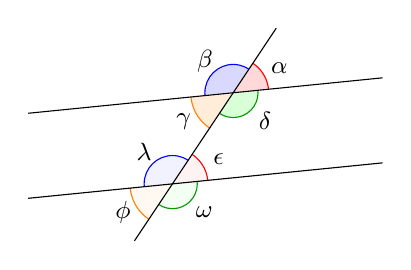
\begin{tikzpicture}[scale=0.9,font=\small, extended line/.style={shorten >=-#1,shorten <=-#1}, extended line/.default=1cm]
\usetikzlibrary{calc, through, intersections}

\begin{scope}
\coordinate (a1) at (0,0);
\coordinate (a2) at (5,0.5);
\coordinate (b1) at (0,1.2);
\coordinate (b2) at (5,1.7);
\coordinate (c1) at (1.5,-0.6);
\coordinate (c2) at (3.5,2.4);

\coordinate (p1) at (intersection of a1--a2 and c1--c2);
\coordinate (p2) at (intersection of b1--b2 and c1--c2);

\begin{scope}
\clip (b1) -- (p2) -- (c2) -- cycle;
\draw[blue, fill=blue!15] (p2) circle (0.4);
\end{scope}
\node[black] at ([shift={(-0.4,0.45)}]p2) {$\beta$};

\begin{scope}
\clip (c2) -- (p2) -- (b2) -- cycle;
\draw[red, fill=red!15] (p2) circle (0.5);
\end{scope}
\node[black] at ([shift={(0.65,0.35)}]p2) {$\alpha$};

\begin{scope}
\clip (c1) -- (p2) -- (b1) -- cycle;
\draw[orange, fill=orange!15] (p2) circle (0.6);
\end{scope}
\node[black] at ([shift={(-0.7,-0.4)}]p2) {$\gamma$};

\begin{scope}
\clip (c1) -- (p2) -- (b2) -- cycle;
\draw[green!60!black, fill=green!15] (p2) circle (0.35);
\end{scope}
\node[black] at ([shift={(0.45,-0.4)}]p2) {$\delta$};

\begin{scope}
\clip (a1) -- (p1) -- (c2) -- cycle;
\draw[blue, fill=blue!5] (p1) circle (0.4);
\end{scope}
\node[black] at ([shift={(-0.4,0.45)}]p1) {$\lambda$};

\begin{scope}
\clip (c2) -- (p1) -- (a2) -- cycle;
\draw[red, fill=red!5] (p1) circle (0.5);
\end{scope}
\node[black] at ([shift={(0.65,0.35)}]p1) {$\epsilon$};

\begin{scope}
\clip (c1) -- (p1) -- (a1) -- cycle;
\draw[orange, fill=orange!5] (p1) circle (0.6);
\end{scope}
\node[black] at ([shift={(-0.7,-0.4)}]p1) {$\phi$};

\begin{scope}
\clip (c1) -- (p1) -- (a2) -- cycle;
\draw[green!60!black, fill=green!5] (p1) circle (0.35);
\end{scope}
\node[black] at ([shift={(0.45,-0.4)}]p1) {$\omega$};


\draw (a1) -- (a2);
\draw (b1) -- (b2);
\draw (c1) -- (c2);

\end{scope}

\end{tikzpicture}

\end{minipage}
\end{esercizio}

\begin{esercizio}
\label{ese:3.19}
Nella figura~\ref{fig:ese3.19} $ABC$ è un triangolo isoscele, $IF$ è parallela a $BC$. Individua tutti gli angoli congruenti all'angolo $A\widehat{B}C$.
\end{esercizio}
\begin{figure}[htb]
\centering% Copyright (c) 2015 Daniele Masini - d.masini.it@gmail.com

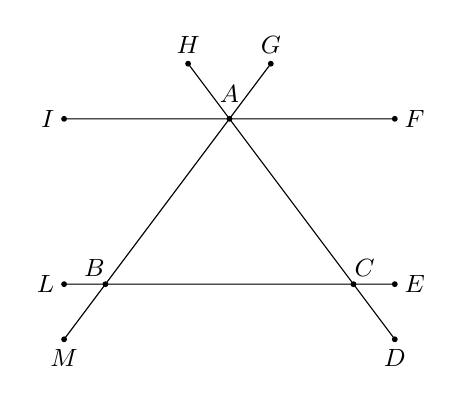
\begin{tikzpicture}[scale=0.7,font=\small, extended line/.style={shorten >=-#1,shorten <=-#1}, extended line/.default=1cm]
\usetikzlibrary{calc, through, intersections}

\begin{scope}
\coordinate (L) at (-3,-3);
\coordinate (E) at (3,-3);
\coordinate (I) at (-3,0);
\coordinate (F) at (3,0);
\coordinate (H) at (-0.75,1);
\coordinate (D) at (3,-4);
\coordinate (G) at (0.75,1);
\coordinate (M) at (-3,-4);

\coordinate (A) at (intersection of H--D and G--M);
\coordinate (B) at (intersection of L--E and G--M);
\coordinate (C) at (intersection of L--E and H--D);

\draw[fill] (I) circle (1.2pt) node[left] {$I$} -- (F) circle (1.2pt) node[right] {$F$};
\draw[fill] (L) circle (1.2pt) node[left] {$L$} -- (E) circle (1.2pt) node[right] {$E$};
\draw[fill] (H) circle (1.2pt) node[above] {$H$} -- (D) circle (1.2pt) node[below] {$D$};
\draw[fill] (G) circle (1.2pt) node[above] {$G$} -- (M) circle (1.2pt) node[below] {$M$};
\draw[fill] (A) circle (1.2pt) node[shift={(0pt,9pt)}] {$A$};
\draw[fill] (B) circle (1.2pt) node[shift={(-4pt,6pt)}] {$B$};
\draw[fill] (C) circle (1.2pt) node[shift={(4pt,6pt)}] {$C$};

\end{scope}

\end{tikzpicture}

\caption{Esercizio~\ref{ese:3.19}}\label{fig:ese3.19}
\end{figure}

\begin{esercizio}
\label{ese:3.20}
Completa ipotesi e tesi e metti in ordine le tre parti della dimostrazione:\\
In un triangolo $ABC$, isoscele su base $AB$, si prendano rispettivamente su $AC$ e $BC$ i punti $D$ ed $E$ equidistanti da $C$. Indicata con $S$ la proiezione di $D$ su $BC$ e con $U$ quella di $E$ su $AC$. Dimostrare che il segmento $US$ è parallelo ad $AB$.\\
~\\
\noindent Ipotesi: $AC\cong \ldots$, $D\in AC$, $E\in \ldots$, $S\in BC$, $DS\perp BC$, $U\in \ldots$, $EU\perp \ldots$\hfill Tesi: $US\parallel AB$.\\
~\\
\noindent\begin{minipage}{.75\textwidth}
\textbf{Parte 1.} I triangoli $CDS$ e $CEU$  hanno: l'angolo $\widehat{C}$ in comune, $CD$ \ldots{} $CE$ per \ldots\ldots{}, $D\widehat{S}C$ \ldots\ldots\ldots{} perché angoli \ldots\ldots{}, quindi tali triangoli sono congruenti per il \ldots\ldots\ldots{}, ne segue $CS \ldots CU$ e pertanto $C\widehat{U}S\cong \ldots$\par

\textbf{Parte 2.} Applicando il teorema sulla somma degli angoli interni ai triangoli $ABC$ e $CUS$, si ha che $C\widehat{U}S + C\widehat{S}U \ldots{} C\widehat{A}B + C\widehat{B}A$ perché supplementari dello stesso angolo $\widehat{C}$, ed essendo $\widehat{A}$ \dots{} $\widehat{B}$ perché \ldots\ldots\ldots{} ed essendo $C\widehat{U}S$ \ldots\ldots{} perché \ldots\ldots\ldots{}, risulta che $C\widehat{A}B$ \ldots{} $C\widehat{U}S$ perché \ldots\ldots\ldots{}\par

\textbf{Parte 3.} Gli angoli $C\widehat{A}B$ e $C\widehat{U}S$ (congruenti perché dimostrato) sono angoli \ldots\ldots rispetto alle rette $AB$ e $US$ tagliate dalla trasversale \ldots, quindi le rette $AB$ e $US$ sono parallele.
\end{minipage}\hfil
\begin{minipage}{.25\textwidth}
\centering% Copyright (c) 2015 Daniele Masini - d.masini.it@gmail.com

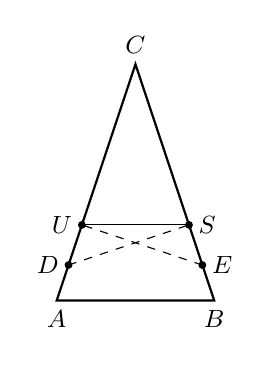
\begin{tikzpicture}[scale=1,font=\small, extended line/.style={shorten >=-#1,shorten <=-#1}, extended line/.default=1cm]
\usetikzlibrary{calc, through, intersections}

\begin{scope}
\coordinate (C) at (0,0);
\coordinate (A) at (-1,-3);
\coordinate (B) at (1,-3);
\coordinate (D) at ($(A)!0.15!(C)$);
\coordinate (E) at ($(B)!0.15!(C)$);
\coordinate (U) at ($(A)!(E)!(C)$);
\coordinate (S) at ($(B)!(D)!(C)$);

\draw[fill] (E) circle (1.2pt) node[right] {$E$};
\draw[fill] (D) circle (1.2pt) node[left] {$D$};
\draw[dashed] (E) -- (U);
\draw[fill] (U) circle (1.2pt) node[left] {$U$};
\draw[dashed] (D) -- (S);
\draw[fill] (S) circle (1.2pt) node[right] {$S$};
\draw (U) -- (S);

\draw[thick] (A) node[below] {$A$} -- (B) node[below] {$B$} -- (C) node[above] {$C$} -- cycle;

\end{scope}

\end{tikzpicture}

\end{minipage}
\end{esercizio}

\begin{esercizio}[Prove invalsi 2005]  %Soluzione: c.
\label{ese:3.21}
$A$, $B$ e $C$ sono tre punti nel piano tali che per i seguenti tre angoli, tutti minori di un angolo piatto, valga la relazione $B\widehat{A}C=A\widehat{B}C+A\widehat{C}B$. Quanto vale $B\widehat{A}C$?
\begin{multicols}{4}
\begin{enumeratea}
\item $70\grado$;
\item $80\grado$;
\item $90\grado$;
\item $100\grado$.
\end{enumeratea}
\end{multicols}
\end{esercizio}

\subsubsection*{Dimostra le seguenti affermazioni sul parallelismo nei poligoni}
\begin{multicols}{2}

\begin{esercizio}
\label{ese:3.22}
Date due rette parallele tagliate da una trasversale, le bisettrici di due angoli corrispondenti (o alterni interni o alterni esterni) sono parallele.
\end{esercizio}

\begin{esercizio}
\label{ese:3.23}
Date due rette parallele tagliate da una trasversale, le bisettrici di due angoli coniugati interni (o coniugati esterni) sono perpendicolari.
\end{esercizio}

\begin{esercizio}
\label{ese:3.24}
Nel triangolo isoscele $ABC$ traccia una parallela alla base $AB$, che incontra i lati obliqui in $D$ ed $E$. Dimostra che anche $DCE$ è un triangolo isoscele.
\end{esercizio}

\begin{esercizio}
\label{ese:3.25}
Se due rette $r$ e $s$ sono incidenti allora lo sono anche due qualsiasi rette $u$ e $v$, con $u \parallel r$ e $v\parallel s$.
\end{esercizio}

\begin{esercizio}
\label{ese:3.26}
Sia $M$ il punto medio del segmento $AB$. Sia $r$ una retta che incontra $AB$ in $M$. Sulla retta $r$ da parti opposte rispetto a $M$ prendi due punti $C$ e $D$ in modo che $AC\parallel BD$. Dimostra che $AC\cong BD$. 
\end{esercizio}

\begin{esercizio}
\label{ese:3.27}
Dal vertice $C$ di un triangolo isoscele $ABC$ conduci la parallela alla base $AB$. Dimostra che tale parallela è bisettrice dell'angolo esterno in $C$ al triangolo.
\end{esercizio}

\begin{esercizio}
\label{ese:3.28}
Sia $ABC$ un triangolo isoscele di base $AB$. Sia $r$ la semiretta di origine $C$ bisettrice dell'angolo formato dal prolungamento di $BC$ e dal lato $AC$. Dimostra che la retta per $AB$ è parallela a $r$.
\end{esercizio}

\begin{esercizio}
\label{ese:3.29}
Dato il triangolo isoscele $ABC$ di base $AB$ e vertice $C$, prolunga la base $AB$ dalla parte di $A$ di un segmento $AD$. Sia $E$ un punto interno all'angolo $D\widehat{A}C$ in modo che $E\widehat{A}D\cong C\widehat{A}B$. Dimostra che $EA\parallel CB$.
\end{esercizio}

\begin{esercizio}
\label{ese:3.30}
Da ciascun vertice di un triangolo $ABC$ traccia la parallela al lato opposto. Detti $D$, $E$ ed $F$ i punti di intersezione delle parallele, dimostra che il triangolo $DEF$ ha gli angoli ordinatamente congruenti a quelli di $ABC$.
\end{esercizio}

\begin{esercizio}
\label{ese:3.31}
Sia $AD$ la bisettrice dell'angolo in $A$ del triangolo $ABC$. Dal punto $D$ traccia la parallela al lato $AB$, essa incontra il lato $AC$ in $E$. Dimostra che il triangolo $EDC$ ha gli angoli ordinatamente congruenti a quelli di $ABC$. Dimostra anche che $ADE$ è un triangolo isoscele.
\end{esercizio}

\begin{esercizio}
\label{ese:3.32}
In un triangolo $ABC$ rettangolo in $A$ traccia l'altezza $AH$ relativa all'ipotenusa. Dimostra che il triangolo $ABH$ ha gli angoli congruenti a quelli di $ABC$.
\end{esercizio}

\begin{esercizio}
\label{ese:3.33}
Sulla base $BC$ di un triangolo isoscele $ABC$ prendi un punto $D$ e traccia da esso la perpendicolare $p$ alla base. La suddetta perpendicolare incontra il lato $AB$ in $E$ e il lato $AC$ in $F$. Dimostra che il triangolo $AFE$ è isoscele.
\end{esercizio}

\begin{esercizio}
\label{ese:3.34}
In un triangolo $ABC$ traccia la bisettrice $AD$ dell'angolo in $A$. Da un punto $N$ del lato $AC$ traccia la parallela alla bisettrice $AD$, essa incontra che retta per $AB$ in $E$ e la retta per $BC$ in $F$. Dimostra che $AEN$ è un triangolo isoscele. Dimostra che $ADC$ e $NFC$ hanno angoli congruenti.
\end{esercizio}

\begin{esercizio}
\label{ese:3.35}
In un triangolo $ABC$ sia $E$ il punto di intersezione della bisettrice dell'angolo in $B$ con il lato $AC$. Sia $D$ un punto del lato $AB$ tale che $DE\cong DB$. Dimostra che $DE\parallel BC$.
\end{esercizio}

\begin{esercizio}
\label{ese:3.36}
In un triangolo $ABC$ traccia le bisettrici agli angoli nei vertici $B$ e $C$. Sia $D$ il punto di intersezione delle bisettrici. Da $D$ traccia la parallela al lato $BC$ e indica con $E$ ed $F$ i punti di intersezione di questa parallela con i lati rispettivamente $AB$ e $AC$. Dimostra che $FE\cong EB+FC$.
\end{esercizio}

\begin{esercizio}
\label{ese:3.37}
Dato il triangolo $ABC$ prolunga il lato $AB$ dalla parte di $A$ di un segmento $AD\cong AB$, prolunga poi il lato $AC$ dalla parte di $A$ di un segmento $AE\cong AC$. Dimostra che $DE\parallel BC$.
\end{esercizio}

\begin{esercizio}
\label{ese:3.38}
Sia $AM$ la mediana di un triangolo $ABC$. Si prolunghi $AM$ dalla parte di $M$ di un segmento $MD$ congruente ad $AM$. Dimostra che $CD$ è parallelo ad $AB$.
\end{esercizio}

\begin{esercizio}
\label{ese:3.39}
Due rette parallele tagliate da una trasversale formano otto angoli, uno di essi è $1/3$ dell'angolo retto. Determina le misure degli altri angoli.
\end{esercizio}

\begin{esercizio}
\label{ese:3.40}
Siano $\alpha$ e $\beta$ due angoli alterni interni formati da due rette parallele tagliate da una trasversale, dimostra che la bisettrice di $\alpha$ è parallela alla bisettrice di $\beta$.
\end{esercizio}

\begin{esercizio}
\label{ese:3.41}
Siano $\alpha$ e $\beta$ due angoli coniugati formati da due rette parallele tagliate da una trasversale, dimostra che la bisettrice di $\alpha$ è perpendicolare alla bisettrice di $\beta$.
\end{esercizio}

\begin{esercizio}
\label{ese:3.42}
Disegna due segmenti $AB$ e $CD$ disposti in modo che si incontrino nel loro punto medio comune $M$. Congiungi $A$ con $D$ e $B$ con $C$, dimostra che $AD$ è parallelo a $CB$.
\end{esercizio}

\begin{esercizio}
\label{ese:3.43}
Disegna un angolo acuto $a\widehat{O}b$ e la sua bisettrice $c$. Disegna su $c$ un punto $P$, disegna poi l'asse del segmento $OP$. Indica con $Q$ e $R$ i punti di intersezione dell'asse rispettivamente con la semiretta $a$ e la semiretta $b$. Dimostra che $OQ$ è parallelo a $RP$.
\end{esercizio}

\begin{esercizio}
\label{ese:3.44}
Disegna un angolo convesso $a\widehat{O}b$ e la sua bisettrice $c$. Disegna su $c$ un punto $P$, disegna poi le perpendicolari $PR$ e $PQ$ rispettivamente alle semirette $a$ e $b$. Dimostra che $c$ è asse del segmento $QR$.
\end{esercizio}

\begin{esercizio}
\label{ese:3.45}
Sia $ABC$ un triangolo equilatero. Traccia una parallela al lato $AB$ che incontra il lato $BC$ in $D$ e $AC$ in $E$. Dimostra che anche il triangolo $CDE$ è equilatero.
\end{esercizio}

\begin{esercizio}
\label{ese:3.46}
Prolunga i lati $AB$ e $AC$ del triangolo $ABC$, entrambi i prolungamenti siano oltre il lato $BC$. Traccia le bisettrici degli angoli esterni ottenuti e sia $P$ il loro punto di incontro. Da $P$ traccia la parallela al lato $BC$, essa incontra $AB$ in $E$ e $AC$ in $F$. Dimostra che $EF=EB+FC$.
\end{esercizio}
\end{multicols}

\begingroup
\hypersetup{linkcolor=black}
\subsubsection*{\ref{sect:angoli_interni_triangolo} - \nameref{sect:angoli_interni_triangolo}}
\endgroup

\begin{esercizio}
\label{ese:3.47}
Vero o Falso?
\begin{enumeratea}
\item La somma degli angoli interni di un triangolo è congruente a un angolo esterno\tab\tab\hfill\boxV\quad\boxF
\item La somma degli angoli interni di un quadrilatero è congruente a 3 angoli piatti\tab\tab\hfill\boxV\quad\boxF
\item La somma degli angoli esterni di un pentagono è congruente a 5 angoli piatti\hfill\boxV\quad\boxF
\item La somma degli angoli interni di un triangolo è congruente a due angoli retti\hfill\boxV\quad\boxF
\item Un triangolo isoscele non può avere un angolo ottuso\hfill\boxV\quad\boxF
\end{enumeratea}
\end{esercizio}

\begin{esercizio}
\label{ese:3.48}
Sia $ABC$ un triangolo equilatero. Si prolunghi $AB$ di un segmento $BD$ congruente al lato stesso e si congiunga $D$ con $C$. Si dimostri che $ACD$ è un triangolo rettangolo.
\end{esercizio}

\begin{esercizio}
\label{ese:3.49}
Calcola la misura degli angoli di un triangolo $ABC$ sapendo che l'angolo interno in $A$ è $4/5$ del relativo angolo esterno e che l'angolo interno in $B$ è la metà dell'angolo interno in $A$.
\end{esercizio}

\begin{esercizio}[I Giochi di Archimede 2003]
\label{ese:3.50}
Sia data una stella a 5 punte inscritta in una circonferenza. Quanto vale la somma degli angoli con vertice nelle punte della stella? 
\end{esercizio}

\begin{esercizio}[I Giochi di Archimede 2005]
\label{ese:3.51}
Nella figura seguente, quanto misura l'angolo $\alpha$?  
\end{esercizio}
\begin{figure}[htb]
\centering% Copyright (c) 2015 Daniele Masini - d.masini.it@gmail.com

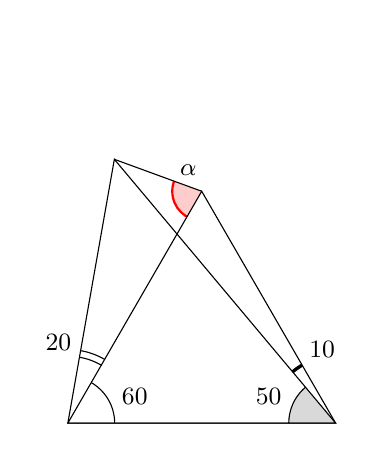
\begin{tikzpicture}[scale=1.7,font=\small, extended line/.style={shorten >=-#1,shorten <=-#1}, extended line/.default=1cm]
\usetikzlibrary{calc, through, intersections}

\begin{scope}
%\coordinate (C) at (0,0);
%\coordinate (A) at (-1,-3);
%\coordinate (B) at (1,-3);
%\coordinate (D) at ($(A)!0.15!(C)$);
%\coordinate (E) at ($(B)!0.15!(C)$);
%\coordinate (U) at ($(A)!(E)!(C)$);
%\coordinate (S) at ($(B)!(D)!(C)$);

%\draw[fill] (E) circle (1.2pt) node[right] {$E$};
%\draw[fill] (D) circle (1.2pt) node[left] {$D$};
%\draw[dashed] (E) -- (U);
%\draw[fill] (U) circle (1.2pt) node[left] {$U$};
%\draw[dashed] (D) -- (S);
%\draw[fill] (S) circle (1.2pt) node[right] {$S$};
%\draw (U) -- (S);

%\draw[thick] (A) node[below] {$A$} -- (B) node[below] {$B$} -- (C) node[above] {$C$} -- cycle;

\path (0,0) coordinate (A) -- ++(60:2) coordinate (B);
\path (B) -- ++(-60:2) coordinate (C);
\path (C) -- (A);

\path (A) -- ++(80:3) coordinate (D1);
\path (C) -- ++(130:3) coordinate (D2);
\coordinate (D) at (intersection of A--D1 and C--D2);

\clip (-0.3,-0.01) -- (-0.3,2) -- (2.1,2) -- (2.1,-0.01) -- cycle;

\begin{scope}
\clip (A) -- (B) -- (C) -- cycle;
\draw (A) circle (0.35);
\node at ([shift={(0.5,0.2)}]A) {$60\grado$};
\end{scope}

\begin{scope}
\clip (A) -- (D) -- (C) -- cycle;
\draw[fill=gray!30] (C) circle (0.35);
\node at ([shift={(-0.5,0.2)}]C) {$50\grado$};
\end{scope}

\begin{scope}
\clip (C) -- (D) -- (B) -- cycle;
\draw[very thick] (C) circle (0.5);
\end{scope}
\node at ([shift={(-0.1,0.55)}]C) {$10\grado$};

\begin{scope}
\clip (A) -- (D) -- (B) -- cycle;
\draw (A) circle (0.5) circle (0.55);
\draw[thick, red, fill=red!20] (B) circle (0.22);
\end{scope}
\node at ([shift={(-0.07,0.6)}]A) {$20\grado$};
\node at ([shift={(-0.1,0.16)}]B) {$\alpha$};

\draw (A) -- (B) -- (C) -- cycle;
\draw (A) -- (D) -- (C) -- cycle;
\draw (D) -- (B);

\end{scope}

\end{tikzpicture}

\caption{Esercizio~\ref{ese:3.31}}\label{fig:ese3.51}
\end{figure}

\begingroup
\hypersetup{linkcolor=black}
\subsubsection*{\ref{sect:generalizzazione_criteri_congruenza_triangoli} - \nameref{sect:generalizzazione_criteri_congruenza_triangoli}}
\endgroup

\begin{esercizio}
\label{ese:3.52}
Vero o Falso?
\begin{enumeratea}
\item Un triangolo rettangolo ha due angoli complementari\hfill\boxV\quad\boxF
\item Due triangoli rettangoli sono congruenti se hanno almeno un lato congruente\hfill\boxV\quad\boxF
\item Due triangoli rettangoli che hanno un cateto in comune sono congruenti\hfill\boxV\quad\boxF
\item Due triangoli rettangoli che hanno l'ipotenusa in comune sono congruenti\hfill\boxV\quad\boxF
\item Due triangoli rettangoli isosceli sono sempre congruenti\hfill\boxV\quad\boxF
\item Due triangoli rettangoli isosceli che hanno un lato in comune sono congruenti\hfill\boxV\quad\boxF
\item Gli angoli acuti di un triangolo rettangolo sono complementari\hfill\boxV\quad\boxF
\end{enumeratea}
\end{esercizio}

\subsubsection*{Dimostra le seguenti affermazioni sui teoremi di congruenza generalizzati}
\begin{multicols}{2}

\begin{esercizio}
\label{ese:3.53}
Dimostra che in triangolo rettangolo gli angoli diversi dall'angolo retto sono acuti.
\end{esercizio}

\begin{esercizio}
\label{ese:3.54}
Dimostra che non può esistere un triangolo rettangolo equilatero.
\end{esercizio}

\begin{esercizio}
\label{ese:3.55}
Due triangoli isosceli sono congruenti se hanno congruenti la base e l'angolo al vertice.
\end{esercizio}

\begin{esercizio}
\label{ese:3.56}
In un triangolo isoscele, le altezze relative ai lati congruenti sono congruenti. 
\end{esercizio}

\begin{esercizio}
\label{ese:3.57}
Due triangoli rettangoli sono congruenti se hanno congruenti un cateto e l'altezza relativa all'ipotenusa.
\end{esercizio}

\begin{esercizio}
\label{ese:3.58}
Due triangoli rettangoli sono congruenti se hanno congruenti un cateto e la mediana relativa ad esso.
\end{esercizio}

\begin{esercizio}
\label{ese:3.59}
Due triangoli rettangoli sono congruenti se hanno congruenti un angolo acuto e la sua bisettrice.
\end{esercizio}

\begin{esercizio}
\label{ese:3.60}
Se due triangoli hanno congruenti due coppie di lati e le mediane relative ai lati rimanenti, allora sono congruenti.
\end{esercizio}

\begin{esercizio}
\label{ese:3.61}
Dimostra che, in un triangolo isoscele, la bisettrice dell'angolo adiacente all'angolo al vertice è parallela alla base.
\end{esercizio}

\begin{esercizio}
\label{ese:3.62}
Dimostra che sono congruenti due triangoli isosceli che hanno gli angoli al vertice congruenti e congruenti le altezze relative a uno dei lati obliqui.
\end{esercizio}

\begin{esercizio}
\label{ese:3.63}
In un triangolo qualsiasi $ABC$ si prenda un qualsiasi punto del lato $AB$ e da esso si tracci la parallela $r$ alla bisettrice dell'angolo interno in $C$. Detto $P$ il punto di intersezione di $r$ con $AC$ e $Q$ il punto di intersezione di $r$ con $BC$, dimostra che $PC\cong QC$.
\end{esercizio}

\begin{esercizio}
\label{ese:3.64}
Sia $D$ il punto di intersezione delle bisettrici degli angoli in $A$ e in $B$ di un triangolo qualsiasi $ABC$. Per $D$ disegna la parallela al lato $AB$, indica con $E$ ed $F$ le intersezioni di questa parallela rispettivamente con il lati $AC$ e $BC$. Dimostra che $AF\cong AE+BF$.
\end{esercizio}

\begin{esercizio}
\label{ese:3.65}
Dimostra che, se per i vertici di un triangolo si conducono le parallele ai lati opposti, queste parallele determinano, assieme al triangolo dato, quattro triangoli congruenti.
\end{esercizio}

\begin{esercizio}
\label{ese:3.66}
Dimostra che in un triangolo isoscele la congiungente i punti medi dei lati congruenti è parallela alla base del triangolo.
\end{esercizio}

\begin{esercizio}
\label{ese:3.67}
Dimostrare che, in un triangolo rettangolo l'altezza relativa all'ipotenusa divide il triangolo in due triangoli rettangolo che hanno tra loro e col triangolo di partenza gli angoli ordinatamente congruenti.
\end{esercizio}

\begin{esercizio}
\label{ese:3.68}
Dato un triangolo $ABC$, si prolunghi il lato $CA$ dalla parte di $A$, si tracci la bisettrice dell'angolo interno di vertice $A$ e si conduca da $B$ la parallela a tale bisettrice, che incontri il prolungamento di $CA$ nel punto $D$. Dimostrare che il triangolo $ADB$ è isoscele.
\end{esercizio}

\begin{esercizio}
\label{ese:3.69}
Dato un angolo convesso $a\widehat{O}b$ traccia la sua bisettrice $c$. Per un punto $P$ della bisettrice traccia la perpendicolare alla bisettrice stessa. Chiama $A$ e $B$ i punto di intersezione della perpendicolare con i lati $a$ e $b$ dell'angolo convesso. Dimostra che $P$ è punto medio di $AB$.
\end{esercizio}

\begin{esercizio}
\label{ese:3.70}
Dato il triangolo isoscele $ABC$, di base $AB$, sul prolungamento dell'altezza relativa ad $AB$ prendi un punto $P$. Traccia le rette $PA$ e $PB$. Dimostra che l'angolo formato dalle rette $PA$ e $CA$ è congruente all'angolo formato dalle rette per $PB$ e $CB$.
\end{esercizio}

\begin{esercizio}
\label{ese:3.71}
Nel triangolo isoscele $ABC$ di vertice $A$ e lati congruenti $AB$ e $AC$, traccia le bisettrici degli angoli alla base. Sia $D$ il loro punto di intersezione. Dimostra che anche il triangolo $DBC$ è isoscele.
\end{esercizio}

\begin{esercizio}
\label{ese:3.72}
Dato un triangolo qualsiasi $ABC$ dimostra che la bisettrice dell'angolo interno in $A$ è perpendicolare alla bisettrice di uno degli angoli esterni in $A$.
\end{esercizio}

\begin{esercizio}
\label{ese:3.73}
Prolunga la mediana $M$ del triangolo $ABC$ di un segmento $MD$. Dimostra che se $AM\cong MD$ allora $BD$ è parallela a $CA$.
\end{esercizio}

\begin{esercizio}
\label{ese:3.74}
Sia $AM$ la mediana di un triangolo $ABC$. Dimostra che se $ABM$ è isoscele il triangolo $ABC$ è rettangolo e viceversa, se il triangolo $ABC$ è rettangolo in $A$ allora $ABM$ è isoscele.
\end{esercizio}

\begin{esercizio}
\label{ese:3.75}
Una retta $t$ incontra due rette $a$ e $b$ rispettivamente in $A$ e $B$. Dal punto medio $M$ di $AB$ traccia una retta che interseca $a$ e $b$ rispettivamente in $C$ e $D$. Dimostra che se $M$ è punto medio di $CD$ allora $a$ e $b$ sono parallele.
\end{esercizio}

\begin{esercizio}
\label{ese:3.76}
Nel triangolo isoscele $ABC$ prolunga la base $AB$ di un segmento $BD$ congruente a $BC$. Dimostra che l'angolo in $C$ esterno al triangolo $ADC$ è il triplo dell'angolo $ADC$.
\end{esercizio}

\begin{esercizio}
\label{ese:3.77}
Dato il triangolo $ABC$ traccia la retta $r$ perpendicolare ad $AB$ passante per $B$, la retta $s$ perpendicolare ad $AB$ passante per $A$, la retta $t$ perpendicolare ad $AC$ passante per $C$. Detti $D$ il punto di intersezione tra $r$ e $t$, $E$ il punto di intersezione tra $s$ e $t$, dimostra che $D\widehat{A}C+C\widehat{B}E+B\widehat{C}E$ è un angolo retto.
\end{esercizio}

\begin{esercizio}
\label{ese:3.78}
Nel triangolo $ABC$ traccia la media $CM$ e il suo prolungamento $MD$ a piacere. Da $A$ conduci la perpendicolare alla mediana che la incontra in $E$, da $B$ conduci un'altra perpendicolare alla mediana che la incontra in $F$. Dimostra che i triangoli $AEM$ e $BFM$ sono congruenti.
\end{esercizio}

\begin{esercizio}
\label{ese:3.79}
Sul prolungamento della base $AB$ di un triangolo isoscele individua un punto $D$ qualsiasi dalla parte di $B$. Traccia la perpendicolare per $D$ a questo prolungamento, essa incontra i lati obliqui del triangolo $AC$ e $BC$ rispettivamente in $E$ e in $F$. Dimostra che il triangolo $CEF$ è isoscele.
\end{esercizio}

\begin{esercizio}
\label{ese:3.80}
Siano $r$ e $s$ due rette incidenti in un punto $O$. Su $r$ prendi da parte opposta rispetto ad $O$ i punti $A$ e $B$ tali che $AO\cong OB$. Su $s$ prendi da parte opposta rispetto ad $O$ i punti $C$ e $D$ tali che $CO\cong OD$. Quale delle seguenti coppie di rette sono parallele? Dimostralo. ($CA\parallel BD$, $CB\parallel AD$)
\end{esercizio}

\begin{esercizio}
\label{ese:3.81}
Sia $ABC$ un triangolo acutangolo. Nel semipiano di origine $AB$ che non contiene $C$ individua un punto $D$ in modo che $B\widehat{A}D\cong C\widehat{B}A$. Dimostra che $CB\parallel AD$. Nell'ipotesi in cui $AD\cong CB$ dimostra che anche $AC\parallel BD$.
\end{esercizio}

\end{multicols}

\begingroup
\hypersetup{linkcolor=black}
\subsubsection*{\ref{sect:disuguaglianze_triangoli} - \nameref{sect:disuguaglianze_triangoli}}
\endgroup

\begin{esercizio}
\label{ese:3.82}
Vero o Falso? 
\begin{enumeratea}
\item Esiste un triangolo i cui lati misurano 10~cm, 3~cm e 15~cm\hfill\boxV\quad\boxF
\item Un triangolo isoscele può essere ottusangolo\hfill\boxV\quad\boxF
\item Dati tre segmenti di cui almeno uno maggiore degli altri è sempre possibile costruire un triangolo che ha lati congruenti ai tre segmenti dati\hfill\boxV\quad\boxF
\item Dai tre segmenti di cui due uguali e uno maggiore degli altri due è sempre possibile costruire un triangolo isoscele che ha lati congruenti ai tre segmenti dati\hfill\boxV\quad\boxF
\item In un triangolo rettangolo l'ipotenusa è minore della somma dei due cateti\hfill\boxV\quad\boxF
\item Un triangolo di perimetro 100~cm non può avere un lato di 60~cm\hfill\boxV\quad\boxF
\item In un triangolo l'angolo che si oppone al lato maggiore è sempre acuto\hfill\boxV\quad\boxF
\item In un triangolo rettangolo i cateti sono sempre congruenti\hfill\boxV\quad\boxF
\item In un triangolo rettangolo l'ipotenusa può essere congruente ad un cateto\hfill\boxV\quad\boxF
\item Un triangolo può avere due lati disuguali e due angoli uguali\hfill\boxV\quad\boxF
\end{enumeratea}
\end{esercizio}

\subsubsection*{Dimostra le seguenti affermazioni}

\begin{multicols}{2}

\begin{esercizio}
\label{ese:3.83}
Sono dati due triangoli $ABC$ e $DEF$ di cui si sa che $\widehat{B}>\widehat{A}$, $\widehat{F}>\widehat{D}$, $BC\cong ED$. Dimostra che $AC>EF$.
\end{esercizio}

\begin{esercizio}
\label{ese:3.84}
Dimostra che in ogni triangolo rettangolo l'ipotenusa è maggiore di ciascun cateto.
\end{esercizio}

\begin{esercizio}
\label{ese:3.85}
Dimostra che in ogni triangolo rettangolo l'ipotenusa è maggiore della semisomma dei cateti.
\end{esercizio}

\begin{esercizio}
\label{ese:3.86}
In un triangolo ottusangolo il lato opposto all'angolo ottuso è maggiore di ciascuno degli altri due lati.
\end{esercizio}

\begin{esercizio}
\label{ese:3.87}
Dimostra che in un triangolo il doppio di un lato è minore del perimetro del triangolo. 
\end{esercizio}

\begin{esercizio}
\label{ese:3.88}
Dimostra che in un triangolo il doppio di una qualsiasi altezza è minore del perimetro del triangolo. 
\end{esercizio}

\begin{esercizio}
\label{ese:3.89}
Dimostra che in un poligono convesso una qualunque diagonale è minore del semiperimetro
\end{esercizio}

\begin{esercizio}
\label{ese:3.90}
Se in un triangolo due mediane sono congruenti, il triangolo è isoscele. 
\end{esercizio}

\begin{esercizio}
\label{ese:3.91}
Se due lati di un triangolo sono disuguali, la mediana uscente dal loro vertice comune forma con il lato opposto angoli disuguali ed è maggiore quello dalla parte del lato maggiore.
\end{esercizio}

\begin{esercizio}
\label{ese:3.92}
In un triangolo ogni lato è minore del semiperimetro.
\end{esercizio}

\begin{esercizio}
\label{ese:3.93}
In un triangolo l'altezza è minore della semisomma dei due lati che hanno un vertice in comune con essa.
\end{esercizio}

\begin{esercizio}
\label{ese:3.94}
In un triangolo, la mediana è minore della semisomma dei due lati che hanno un vertice in comune con essa.
\end{esercizio}

\begin{esercizio}
\label{ese:3.95}
In un triangolo $ABC$ traccia la bisettrice $BE$ dell'angolo in $B$. Dimostra che $AB>AE$. (Per la dimostrazione utilizza il teorema dell'angolo esterno).
\end{esercizio}

\begin{esercizio}
\label{ese:3.96}
Nel triangolo $ABC$ traccia la mediana $AM$. Dimostra che se $AC$ è maggiore di $AB$ allora l'angolo $A\widehat{M}C$ è maggiore dell'angolo $A\widehat{M}B$.
\end{esercizio}

\begin{esercizio}
\label{ese:3.97}
Nel triangolo $ABC$ prendi un punto $D$ interno al triangolo. Dimostra che il perimetro del triangolo $ADB$ è minore del perimetro del triangolo $ABC$. (Prolunga il lato $AD$ fino a incontrare il lato $BC$ in $E$. Ragionando opportunamente sui triangoli che si vengono a formare dimostra che $AD+DB<AC+CB$).
\end{esercizio}

\begin{esercizio}
\label{ese:3.98}
Esternamente al triangolo $ABC$ prendi un punto $D$. Congiungi $D$ con $A$, con $B$ e con $C$. Dimostra che il perimetro di $ABC$ è minore del doppio della somma delle distanze di $D$ dai tre vertici del triangolo.
\end{esercizio}

\begin{esercizio}
\label{ese:3.99}
Nel triangolo $ABC$ traccia la mediana $AM$ relativa al lato $BC$, dimostra che $AM$ è minore della semisomma degli altri due lati $AB$ e $AC$. (Prolunga la mediana di un segmento congruente alla mediana stessa.)
\end{esercizio}

\begin{esercizio}
\label{ese:3.100}
In ogni triangolo, la somma delle mediane è minore del perimetro e maggiore del semiperimetro.
\end{esercizio}

\begin{esercizio}
\label{ese:3.101}
Dimostra che in un triangolo acutangolo, la somma delle altezze è minore del perimetro e maggiore del semiperimetro.
\end{esercizio}

\begin{esercizio}
\label{ese:3.102}
Dato un triangolo $ABC$ in cui $AB<AC$ traccia l'altezza $AH$ relativa alla base $BC$. Dimostra che l'angolo $H\widehat{A}C$ è maggiore dell'angolo $H\widehat{A}B$.
\end{esercizio}

\begin{esercizio}
\label{ese:3.103}
Dato il triangolo isoscele $ABC$ unisci il vertice $A$ con un punto $D$ della base $BC$. Dimostra che $AD$ è minore di ciascuno dei due lati congruenti, $AB$ e $AC$.
\end{esercizio}

\begin{esercizio}
\label{ese:3.104}
Dimostra in un poligono convesso, una qualunque diagonale è minore del semiperimetro.
\end{esercizio}

\begin{esercizio}
\label{ese:3.105}
In un triangolo $ABC$ si ha che $AB>AC$. Si tracci la bisettrice $AD$ dell'angolo in $A$. Si dimostri che $A\widehat{D}B>A\widehat{D}C$.
\end{esercizio}

\begin{esercizio}
\label{ese:3.106}
Due triangoli rettangoli hanno un cateto in comune e l'angolo opposto al cateto in comune è maggiore nel primo triangolo. Dimostra che l'ipotenusa del primo triangolo è minore di quella del secondo.
\end{esercizio}

\begin{esercizio}
\label{ese:3.107}
Dimostra che in ogni triangolo la somma dei tre lati è sempre maggiore del doppio di un lato.
\end{esercizio}

\begin{esercizio}
\label{ese:3.108}
Sia $AM$ la mediana di un triangolo generico $ABC$. Dimostra che se $AB>AC$ allora $A\widehat{M}C<A\widehat{M}B$.
\end{esercizio}

\begin{esercizio}
\label{ese:3.109}
Disegna un punto $D$ interno a un triangolo $ABC$ qualsiasi. Dimostra che $B\widehat{D}C>B\widehat{A}C$.
\end{esercizio}

\begin{esercizio}
\label{ese:3.110}
Sui lati $AB$, $BC$, $CA$ di un triangolo $ABC$ qualsiasi, scegli a caso tre punti, rispettivamente $D$, $E$ ed $F$. Dimostra che il perimetro di $ABC$ è maggiore del perimetro di $DEF$.
\end{esercizio}

\begin{esercizio}
\label{ese:3.111}
Un quadrilatero $ABCD$ si compone di un triangolo isoscele $ABC$ di base $BC$ e di un triangolo rettangolo isoscele $ACD$ con l'angolo retto in $C$. Dimostra che se l'angolo in $A$ del triangolo isoscele è acuto allora $BC<CD$, se l'angolo in $A$ del triangolo isoscele è ottuso risulta $CD<BC$.
\end{esercizio}

\end{multicols}

\begin{esercizio}[Prove invalsi 2004]
\label{ese:3.112}
~\\
\noindent\begin{minipage}{0.6\textwidth}
Le rette $r$ ed $s$ sono tagliate dalla trasversale $t$. Quale delle seguenti condizioni permette di stabilire, per qualunque posizione di $t$, che $r$ ed $s$ sono parallele?\\
Gli angoli \ldots{}
\begin{enumeratea}
\item 1 e 5 sono supplementari;
\item 2 e 8 sono uguali;
\item 3 e 7 sono supplementari;
\item 4 e 7 sono uguali.
\end{enumeratea}
\end{minipage}\hfil
\begin{minipage}{0.4\textwidth}
\centering% Copyright (c) 2015 Daniele Masini - d.masini.it@gmail.com

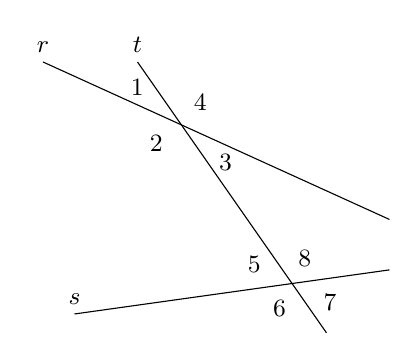
\begin{tikzpicture}[scale=0.8,font=\small, extended line/.style={shorten >=-#1,shorten <=-#1}, extended line/.default=1cm]
\usetikzlibrary{calc, through, intersections}

\begin{scope}
\coordinate (s1) at (0,0);
\coordinate (s2) at (5,0.7);
\coordinate (r1) at (-0.5,4);
\coordinate (r2) at (5,1.5);
\coordinate (t1) at (4,-0.3);
\coordinate (t2) at (1,4);

\coordinate (p1) at (intersection of s1--s2 and t1--t2);
\coordinate (p2) at (intersection of r1--r2 and t1--t2);

\node[black] at ([shift={(-0.7,0.6)}]p2) {$1$};
\node[black] at ([shift={(0.3,0.35)}]p2) {$4$};
\node[black] at ([shift={(-0.4,-0.3)}]p2) {$2$};
\node[black] at ([shift={(0.7,-0.6)}]p2) {$3$};

\node[black] at ([shift={(-0.6,0.3)}]p1) {$5$};
\node[black] at ([shift={(0.2,0.4)}]p1) {$8$};
\node[black] at ([shift={(-0.2,-0.4)}]p1) {$6$};
\node[black] at ([shift={(0.6,-0.3)}]p1) {$7$};

\draw (r1) node[above] {$r$} -- (r2);
\draw (s1) node[above] {$s$} -- (s2);
\draw (t1) -- (t2) node[above] {$t$};

\end{scope}

\end{tikzpicture}

\end{minipage}
\end{esercizio}

\begin{esercizio}[Prove invalsi 2006]
\label{ese:3.113}
Per un triangolo ottusangolo qualsiasi, quale delle seguenti affermazioni è vera?
\begin{enumeratea}
\item La somma dei suoi due angoli più piccoli è minore dell'angolo più grande.
\item Il punto di incontro degli assi dei lati è certamente interno al triangolo.
\item Il triangolo è necessariamente isoscele.
\item Il triangolo può essere rettangolo.
\end{enumeratea}
\end{esercizio}

\begin{esercizio}[Prove invalsi 2006]
\label{ese:3.114}
~\\
\noindent\begin{minipage}{0.65\textwidth}
$r$ ed $s$ sono due rette parallele tagliate da una trasversale $t$. Quale tra le seguenti proposizioni è vera qualunque sia la posizione di $t$?
Gli angoli $\alpha$ e $\beta$ sono \ldots{}
\begin{enumeratea}
\item supplementari;
\item uguali;
\item complementari;
\item corrispondenti.
\end{enumeratea}
\end{minipage}\hfil
\begin{minipage}{0.35\textwidth}
\centering% Copyright (c) 2015 Daniele Masini - d.masini.it@gmail.com

\begin{tikzpicture}[scale=0.8,font=\small, extended line/.style={shorten >=-#1,shorten <=-#1}, extended line/.default=1cm]
\usetikzlibrary{calc, through, intersections}

\begin{scope}
\coordinate (s1) at (0,0);
\coordinate (s2) at (5,0);
\coordinate (r1) at (0,2);
\coordinate (r2) at (5,2);
\coordinate (t1) at (1,-0.7);
\coordinate (t2) at (3.5,2.7);

\coordinate (p1) at (intersection of s1--s2 and t1--t2);
\coordinate (p2) at (intersection of r1--r2 and t1--t2);

\node[black] at ([shift={(-0.6,-0.3)}]p2) {$\alpha$};

\node[black] at ([shift={(0.1,-0.4)}]p1) {$\beta$};

\draw (r1) -- (r2) node[above] {$r$};
\draw (s1) -- (s2) node[above] {$s$};
\draw (t1) -- (t2) node[left] {$t$};

\end{scope}

\end{tikzpicture}

\end{minipage}
\end{esercizio}

\begin{esercizio}[Prove invalsi 2004]
\label{ese:3.115}
In un triangolo, le misure dei lati sono $a$, $b$ e $c$, con $a = b < c$. Detti $\alpha$, $\beta$ e $\gamma$ gli angoli interni del triangolo, rispettivamente opposti ai lati $a$, $b$ e $c$, quale delle seguenti affermazioni è vera?
\begin{multicols}{4}
\begin{enumeratea}
\item $\alpha = \gamma$;
\item $\beta = \gamma$;
\item $\gamma > \alpha$;
\item $\alpha > \beta$.
\end{enumeratea}
\end{multicols}
\end{esercizio}

\begin{esercizio}[Prove invalsi 2010]
\label{ese:3.116}
Un triangolo ha un lato di 6~cm e uno di 10~cm. Quale tra le seguenti non può essere la misura della lunghezza del terzo lato?
\begin{multicols}{4}
\begin{enumeratea}
\item $\np{6,5}$~cm;
\item 10~cm;
\item $\np{15,5}$~cm;
\item 17~cm.
\end{enumeratea}
\end{multicols}
\end{esercizio}

\pagebreak

\begin{esercizio}[Prove invalsi 2005]
\label{ese:3.117}
In un triangolo isoscele l'angolo al vertice è metà dell'angolo alla base. Quanto misurano gli angoli del triangolo?
\begin{multicols}{4}
\begin{enumeratea}
\item $72\grado$, $72\grado$, $36\grado$;
\item $30\grado$, $60\grado$, $90\grado$;
\item $36\grado$, $36\grado$, $72\grado$;
\item $90\grado$, $45\grado$, $45\grado$.
\end{enumeratea}
\end{multicols}
\end{esercizio}


\subsection{Risposte}

\begingroup
\hypersetup{linkcolor=black}

\paragraph{\ref{ese:3.1}.}
a)~F,\quad b)~F,\quad c)~F,\quad d)~F,\quad e)~F,\quad f)~V.

\paragraph{\ref{ese:3.10}.}
a)~V,\quad b)~F,\quad c)~F,\quad d)~V.

\paragraph{\ref{ese:3.11}.}
a.

\paragraph{\ref{ese:3.15}.}
a)~F,\quad b)~F,\quad c)~F,\quad d)~F,\quad e)~V,\quad f)~V,\quad g)~F,\quad h)~F,\quad i)~F,\quad j)~F,\quad k)~F,\quad l)~V.

\paragraph{\ref{ese:3.18}.}
$\alpha=\dfrac{1}{3}\pi$, $\beta=\dfrac{2}{3}\pi$, $\gamma=\dfrac{1}{3}\pi$, $\delta=\dfrac{2}{3}\pi$, $\epsilon=\dfrac{1}{3}\pi$, $\lambda=\dfrac{2}{3}\pi$, $\phi=\dfrac{1}{3}\pi$, $\omega=\dfrac{2}{3}\pi$.

\paragraph{\ref{ese:3.21}.}
c.

\paragraph{\ref{ese:3.47}.}
a)~F,\quad b)~F,\quad c)~F,\quad d)~V,\quad e)~F.

\paragraph{\ref{ese:3.49}.}
$60\grado$, $30\grado$, $90\grado$.

\paragraph{\ref{ese:3.50}.}
$180\grado$.

\paragraph{\ref{ese:3.51}.}
$80\grado$.

\paragraph{\ref{ese:3.52}.}
a)~V,\quad b)~F,\quad c)~F,\quad d)~V,\quad e)~F,\quad f)~V,\quad g)~V.

\paragraph{\ref{ese:3.82}.}
a)~F,\quad b)~V,\quad c)~F,\quad d)~F,\quad e)~V,\quad f)~V,\quad g)~F,\quad h)~F,\quad i)~F,\quad j)~V.

\paragraph{\ref{ese:3.112}.}
b.

\paragraph{\ref{ese:3.113}.}
a.

\paragraph{\ref{ese:3.114}.}
a.

\paragraph{\ref{ese:3.115}.}
c.

\paragraph{\ref{ese:3.116}.}
d.

\paragraph{\ref{ese:3.117}.}
a.

\endgroup
